\section{Resolución de artefactos}

\SectionPage

\begin{frame}{Sobreestimación}
    
    Cuando tratamos \textit{funciones de distancia con signo no exactas}, utilizaremos el término \enquote{sobreestimar} cuando se supera la distancia mínima real a la superficie a lo que llamaremos \enquote{artefacto}.
    El rayo trazado se encuentra dentro de la superficie o  el rayo atraviese una superficie. 
    
    \vfill
    
    \begin{columns}[onlytextwidth]
        \begin{column}{0.45\textwidth}
            \begin{figure}[H]
              \centering
              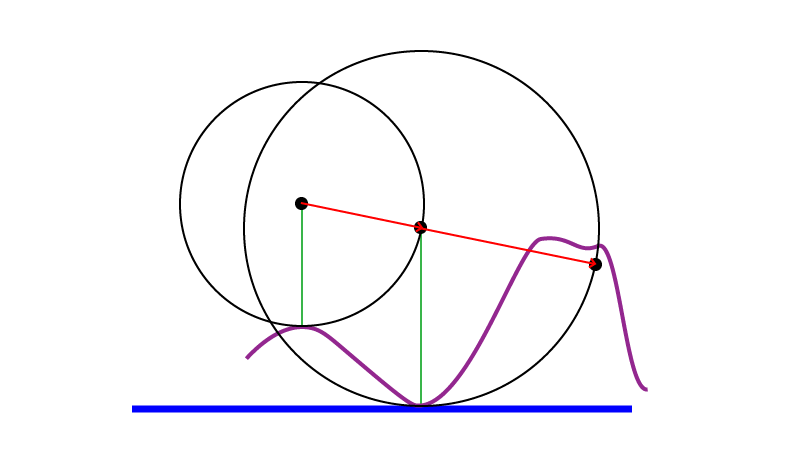
\includegraphics[width=1.0\textwidth]{imagenes/estimation/sobreestimar-interior.png}
              %\caption{Fragment shader y Lanzamiento de rayos para el trazado de una escena}
            \end{figure}
            {\small 1) Estimación dentro de la superficie.}
        \end{column}
        
        \begin{column}{0.45\textwidth}
            \begin{figure}[H]
              \centering
              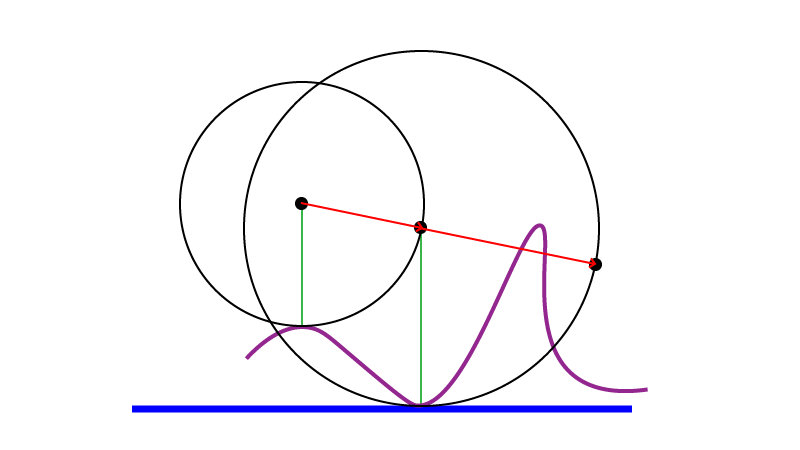
\includegraphics[width=1.0\textwidth]{imagenes/estimation/sobreestimar-exterior.png}
              %\caption{Ejemplo del algoritmo \textit{Spheremarching}}
            \end{figure}
            {\small 2) Estimación fuera de la superficie.}
        \end{column}
        
    \end{columns}

\end{frame}


\begin{frame}{Solución para la sobreestimación}
    
    Vamos a modificar la condición de parada impuesta que definía \enquote{estar sobre la isosuperficie}. Ahora, diremos que estamos sobre una superficie, si y solo si, \( \vert f(\Vec{rayo_{n}}) \vert < \epsilon\), así, si nos encontramos dentro, deberá salir del objeto, gracias al signo de la distancia.
    
    \vfill
    
    \begin{enumerate}
        \item Incrementar el número de iteraciones para nuestro algoritmo.
        \item Escalar \(k\in[0,1]\) el radio de la bola, es decir, la distancia más corta a la superficie.
        \[d'_{n}=d_{n-1} + f(\Vec{p}_{n-1})\cdot k \leq d_{n}\]
    \end{enumerate}
    
    \vfill
    
    \begin{columns}[onlytextwidth]
        \begin{column}{0.45\textwidth}
            \begin{figure}[H]
              \centering
              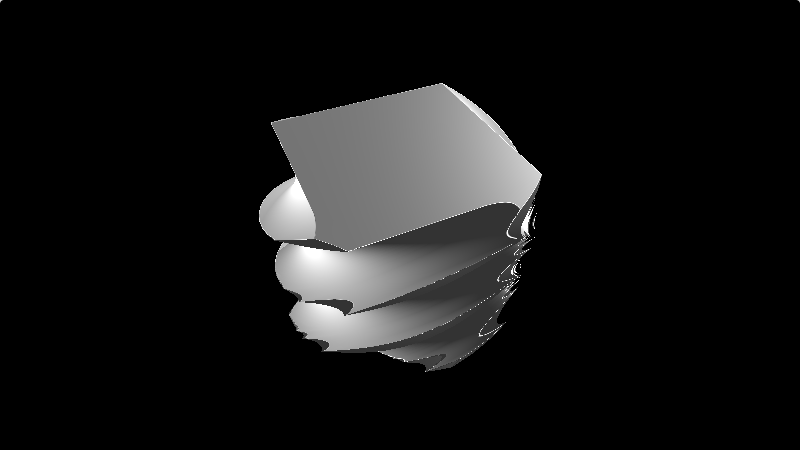
\includegraphics[width=1.0\textwidth]{imagenes/sdf/3d/sdf_twist.png}
              %\caption{Fragment shader y Lanzamiento de rayos para el trazado de una escena}
            \end{figure}
            {\small 1) Estimación dentro de la superficie.}
        \end{column}
        
        \begin{column}{0.45\textwidth}
            \begin{figure}[H]
              \centering
              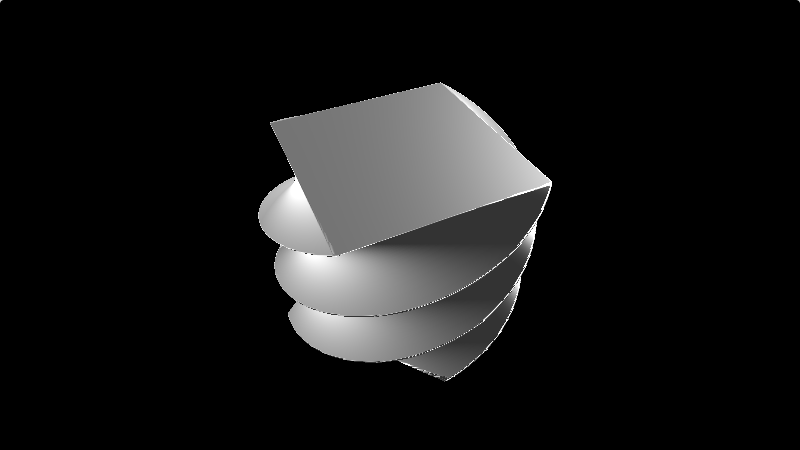
\includegraphics[width=1.0\textwidth]{imagenes/estimation/sobreestimacion_50.png}
              %\caption{Ejemplo del algoritmo \textit{Spheremarching}}
            \end{figure}
            {\small 2) Estimación fuera de la superficie.}
        \end{column}
        
    \end{columns}
    
\end{frame}



\begin{frame}{Subestimación}
    
    Este tipo de estimación puede ocurrir tanto en \textit{funciones de distancia con signo exactas como inexactas}. Cuando el \textit{Marcher} finaliza consumiendo todas las iteraciones disponibles, es decir, en la \textbf{Tercera condición}. Suele ocurrir cuando el rayo pasa de manera paralela, muy cerca a una superficie con \(f(\Vec{rayo_{n}}) \ge \epsilon\). La solución trivial es incrementar el número de iteraciones.
    
    \vfill
    
    \begin{figure}[H]
      \centering
      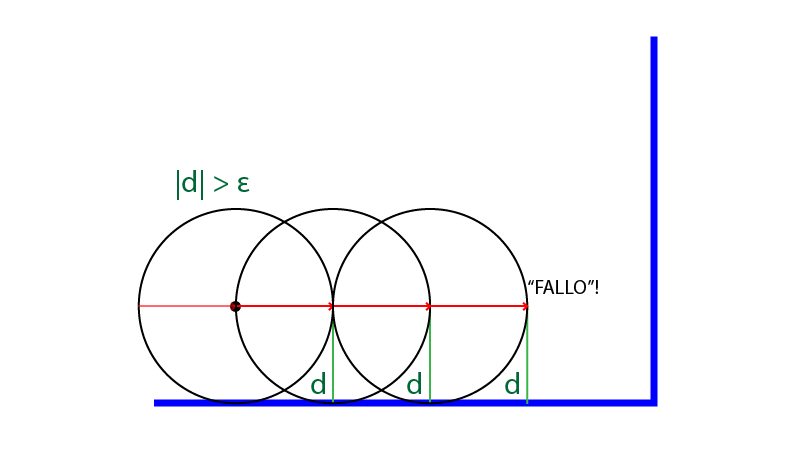
\includegraphics[width=0.8\textwidth]{imagenes/estimation/subestimacion.png}
      %\caption{Fragment shader y Lanzamiento de rayos para el trazado de una escena}
    \end{figure}
    
\end{frame}